%
% Tesi D.S.I. - modello preso da
% Stanford University PhD thesis style -- modifications to the report style
%
%%%%%%%%%%%%%%%%%%%%%%%%%%%%%%%%%%%%%%%%%%%%%%%%%%%%%%%%%%%%%%%%%%%%%%%%%%%
%                                                                         %
%			TESI DOTTORATO                                                   %
%			______________                                                   %
%                                                                         %
%			AUTORE: Elena Pagani                                             %
%                                                                         %
%			Ultima revisione: 7.X.1998                                       %
%           correzioni atrent                                             %
%%%%%%%%%%%%%%%%%%%%%%%%%%%%%%%%%%%%%%%%%%%%%%%%%%%%%%%%%%%%%%%%%%%%%%%%%%%
%
%
\documentclass[a4paper,12pt]{report}
%    \renewcommand{\baselinestretch}{1.6}      % interline spacing
%
% \includeonly{}
%
%			PREAMBOLO
%
\usepackage[a4paper]{geometry}
\usepackage{amssymb,amsmath,amsthm}
\usepackage{graphicx}
\usepackage{url}
\usepackage{hyperref}
\usepackage{epsfig}
\usepackage[italian]{babel}
\usepackage{setspace}
\usepackage{tesi}

% Aggiunti da me
\hypersetup{hidelinks}
\usepackage{subcaption}
\usepackage{float}


% per le accentate
\usepackage[utf8]{inputenc}
%
\newtheorem{myteor}{Teorema}[section]
%
\newenvironment{teor}{\begin{myteor}\sl}{\end{myteor}}
%
%
%			TITOLO
%
\begin{document}
\title{Tecniche di machine learning per la classificazione di reperti archeologici}
\author{Pietro Scuttari}
\dept{Corso di Laurea in informatica} 
\anno{2020-2021}
\matricola{922822}
\relatore{Prof.ssa Anna Maria Zanaboni}
\correlatore{Prof. Dario Malchiodi}
%
%        \submitdate{month year in which submitted to GPO}
%		- date LaTeX'd if omitted
%	\copyrightyear{year degree conferred (next year if submitted in Dec.)}
%		- year LaTeX'd (or next year, in December) if omitted
%	\copyrighttrue or \copyrightfalse
%		- produce or don't produce a copyright page (false by default)
%	\figurespagetrue or \figurespagefalse
%		- produce or don't produce a List of Figures page
%		  (false by default)
%	\tablespagetrue or \tablespagefalse
%		- produce or don't produce a List of Tables page
%		  (false by default)
% 
%			DEDICA
%
\beforepreface
% \prefacesection{}
% 		{\hfill \Large {\sl dedicato a \dots}}
% 
%			PREFAZIONE
%
\prefacesection{Prefazione}
\section{Descrizione del problema}
Questo elaborato descrive il lavoro fatto durante un tirocinio nato dalla
collaborazione del dipartimento di informatica e il corso in Scienze e
tecnologie per lo studio e la conservazione dei beni culturali e dei supporti
dell'informazione. Sono stati ritrovati una serie di reperti archeologici nel
sito della necropoli di Cerveteri ma non tutti sono originali del luogo e il
nostro obbiettivo è quello di classificare i reperti separando quelli originali
del luogo da quelli di origine esterna. Per fare ciò il corso di beni culturali
ci ha fornito un database di dati ottenuti dall'analisi di composizioni sui
reperti. Su questo database abbiamo usato diversi algoritmi di classificazioni
basati su modelli di machine learning. Ognuno di questi ha prodotto un'ipotesi
sull'origine dei reperti e combinando tutte le stime siamo riusciti a produrre
una classificazione complessiva per tutti i reperti del database.

% L'obbiettivo di questo progetto è riuscire a risalire all'origine geografica di
% alcuni reperti archeologici ritrovati nel sito della necropoli di cerveteri
% utilizzando tecniche di machine learning. Per ogni reperto archeologico sono
% state eseguite delle analisi di composizione producendo così un database su cui
% poter eseguire i diversi algoritmi utilizzati lavorando principalmente su un
% sottoinsieme di questi reperti di cui è nota la provenienza per poi applicare i
% modelli generati al database completo.


%
%
%			ORGANIZZAZIONE
\section{Organizzazione del documento}
\label{organizzazione}
La tesi \`e organizzata come segue:
\begin{itemize}
	\item Nel capitolo 1 viene introdotto il progetto introducendo i concetti
	principali e gli algoritmi utilizzati.

	\item Nel capitolo 2 sono approfonditi i dati e come sono stati utilizzati
	gli algoritmi

\end{itemize}
%
%			RINGRAZIAMENTI
%
% \prefacesection{Ringraziamenti}
% asdjhgftry.
% \afterpreface
% 
% 
%			CAPITOLO 1: Introduzione
\chapter[Algoritmi di ML e classificazione]{Algoritmi di machine learning e di classificazione}
\label{cap1}

\section{Che cos'è il machine learning}

Per machine learning si intende un diverso approccio alla soluzione di problemi in
informatica. Nell'approccio tradizionale per risolvere un problema creiamo un
algoritmo specificando passo per passo tutte le operazioni necessarie per
arrivare alla soluzione. Al contrario con il machine learning vogliamo che il
programma autonomamente ricrei un modello del problema a partire da una serie di
istanze del problema stesso in un processo detto allenamento. Il modello creato
avendo solo poche istanze su cui basarsi non sarà sempre accurato nella
soluzione ma tipicamente riusciamo a raggiungere una buona approssimazione. 

% Machine learning è un nome che include una varietà di algoritmi che, al
% contrario di algoritmi tradizionali, non specificano passo per passo come
% risolvere un certo problema ma autonomamente creano un modello del problema, in
% un processo detto allenamento, a partire da alcune istanze di questo. Otteniamo
% così un un modello ovvero una rappresentazione matematica semplificata del
% problema originale che usiamo per approssimare una soluzione per ogni istanza
% possibile del problema. 

Per creare un buon modello è quindi necessario avere una buona quantità di
istanze ognuna composta da più valori, detti caratteristiche, le istanze vengono
tipicamente divise in due parti: l'insieme di training e l'insieme di di test.
Il primo viene usato per l'allenamento del modello e il secondo per valutare le
sue prestazioni. È importante che questi rimangano separati altrimenti il
modello sarebbe facilitato da aver gia visto i dati durante l'allenamento e non
potremmo valutare accuratamente le prestazioni reali. 

Esistono due principali sottoinsiemi di algoritmi, quelli detti di apprendimento
supervisionato e quelli di apprendimento non supervisionato. Nel primo caso il
training set è etichettato ovvero per ogni istanza è specificata la soluzione,
detta etichetta, corrispondente, al contrario questa informazione non è presente
per l'apprendimento non supervisionato. Il primo caso è tipicamente più semplice
data l'informazione ulteriore disponibile e è anche quello principalmente
utilizzato in questo progetto.

\section{Cosa sono i problemi di classificazione}

I problemi di classificazione consistono nel produrre un algoritmo, detto
classificatore, in grado associare a un istanza di input una o più categorie,
come ad esempio una mail a "spam" o "non spam". Questo tipo di problema si presta
molto alle tecniche di machine learning infatti spesso è difficile programmare
manualmente stretti criteri per la classificazione ma è possibile lasciare al
calcolatore questo compito fornendo solo una serie di esempi corretti da cui
possa imparare.

\section{Reti neurali}

\begin{figure}
	\centering
	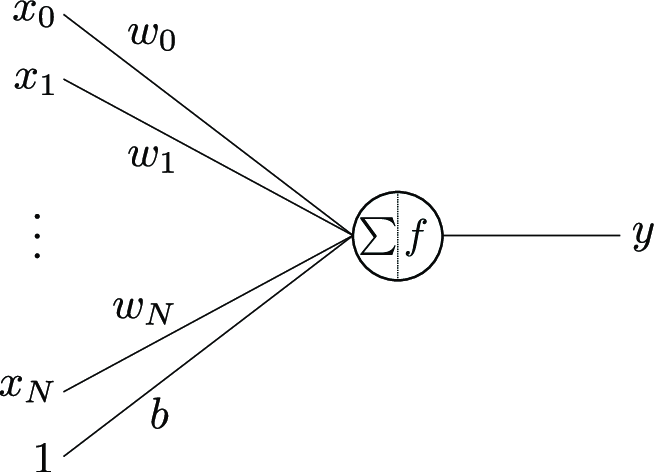
\includegraphics[width = 0.4\textwidth]{Immagini/MLP neurone.png}
	\caption{Rappresentazione di un neurone in una rete neurale. Le $x$
	rappresentano gli input del neurone, le $w$ i loro pesi, $f$ la funzione di
	attivazione e $y$ l'output (fonte \cite{immagine neurone})}
\end{figure}

Le reti neurali sono una famiglia di modelli, ispirati alle reti neuronali
biologiche, composti da una serie di neuroni collegati fra loro. Un
neurone, come quello mostrato nella figura 1, non è altro che una semplice
funzione che moltiplica ogni input $x_i$ per un certo peso $w_i$, i risultati
vengono sommati e usati come argomento di una funzione di attivazione $f$ che
produce l'output $y$ del neurone:

$$
y = f\left(\sum_i x_i w_i\right).
$$

Spesso è utilizzata una funzione di attivazione che produce risultati compresi
tra 0 e 1 in modo da uniformare gli input del neurone successivo, questo non è
sempre il caso specialmente nell'ultimo strato di neuroni.

Il modo in cui i neuroni sono collegati tra loro è detto topologia e nel caso
utilizzato in questo progetto, un modello detto percettrone multistrato, i
neuroni sono organizzati in diversi strati collegati fra loro in modo che
l'output di ogni strato funge da input per il successivo. Il primo strato è
detto strato di input: qui abbiamo tanti neuroni quante le caratteristiche
dei dati in ingresso al modello, ogni neurone elabora una caratteristica secondo
la propria funzione e invia l'output a tutti i neuroni dello strato successivo. In
seguito abbiamo una serie di strati detti nascosti in cui a ogni livello i
neuroni ricevono l'output di tutti i neuroni nel livello precedente e inviano il
loro risultato a tutti i neuroni del livello successivo. L'ultimo livello è
quello di output in cui i neuroni ricevono l'output dall'ultimo strato nascosto e
restituiscono la soluzione del problema. La dimensione del livello di output è determinata
dalla codifica della soluzione, ad esempio in un problema di classificazione
avremmo tanti neuroni in uscita quante categorie possibili per la
classificazione oppure se dobbiamo generare un immagine potremmo avere tanti
neuroni quanti i pixel dell'immagine.

\begin{figure}
	\centering
	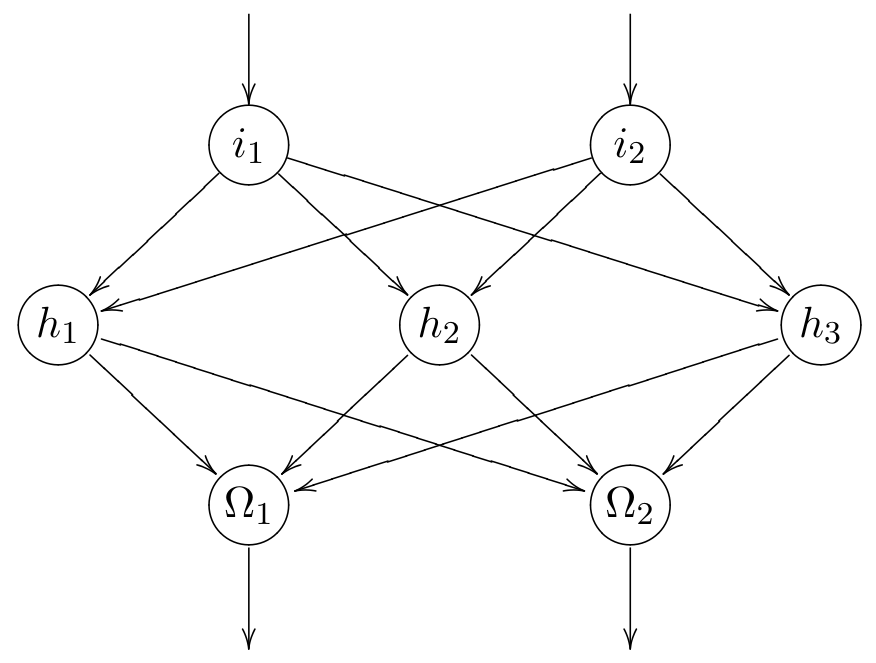
\includegraphics[width = 0.4\textwidth]{Immagini/MLP diagramma.png}
	\captionof{figure}{Semplice rappresentazione di un percettrone multistrato
	con due neuroni di input ($i_1$ e $i_2$), tre in un singolo strato nascosto ($h_1
	... h_3$) e due in output ($\Omega_1$ e $\Omega_2$) (fonte \cite{Intro to nn})}
\end{figure}

I parametri delle funzioni dei neuroni, i pesi e i parametri di $f$, sono
inizializzati con dei valori casuali e vengono perfezionati durante
l'apprendimento il quale, nel nostro caso, sarà supervisionato. A ogni istanza
di input si confronta l'output della rete con l'etichetta del dato correggendo
poi i valori dei parametri dei neuroni per far avvicinare la risposta della rete
a quella corretta. Il processo viene ripetuto iterativamente fino a che viene
raggiunto un criterio di arresto come un certo numero di iterazioni, una soglia
sull'errore o una soglia sul rateo di miglioramento. 

All'utente viene lasciato il controllo di quelli che vengono detti iperparametri
ovvero i parametri che controllano il funzionamento della rete neurale e che non
vengono modificati durante l'apprendimento. Alcuni esempi sono la topologia
della rete, la funzione di attivazione, la dimensione del passo di apprendimento
eccetera.

%Cost function
%Gradiente
%Backpropagation

\section{K-nearest neighbors}

K-nearest neighbors è uno dei modelli più semplici tra quelli usati: invece che
creare un modello interno del problema questo semplicemente memorizza i dati di
training e per classificare una nuova istanza calcola quali sono i $K$ valori
memorizzati più vicini e restituisce l'etichetta più frequente tra questi.

Uno dei possibili problemi è la poca uniformità dei dati: se i valori più vicini
selezionati sono molto distanti dal punto che stiamo cercando di classificare
potrebbero non essere rilevanti per la classificazione. Per ovviare a questo
problema è possibile pesare il calcolo per l'etichetta più frequente con la
distanza dei punti dando quindi meno importanza ai punti più distanti.

Un importante iperparametro di cui abbiamo controllo è $K$ ovvero il numero di
dati di training da considerare per calcolare l'etichetta più probabile. La
scelta corretta dipende dal nostro dataset: ci serve un $K$ sufficientemente
grande per avere un numero di punti statisticamente significativo ma non troppo
altrimenti prenderemmo punti troppo distanti e quindi della categoria sbagliata.


Un valore maggiore dihh
$K$ sarà utile per superare il rumore statistico dei nostri dati ma produrrà una
distinzione meno netta tra le categorie.



\section{Macchine a vettori di supporto}

L'obbiettivo di una macchina a vettori di supporto (SVM) è trovare un iperpiano
che separi i dati di training nelle corrette categorie cercando di massimizzare
il margine, ovvero la distanza tra l'iperpiano e i dati più vicini di ogni
categoria. Fatto questo per classificare un nuovo dato basterà vedere da che
parte dell'iperpiano si trova.

\begin{figure}[h]
	\centering
	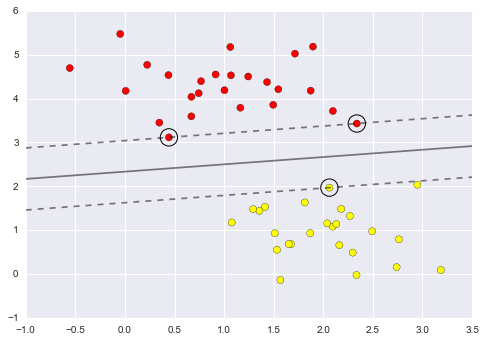
\includegraphics[width =0.6\textwidth]{Immagini/SVM margine.png}
	\caption{Esempio di iperpiano con i limiti del margine evidenziati (fonte \cite{Data science handbook})} 
	
\end{figure}

A volte i dati sono posizionati in modo da non essere separabili linearmente, in
questi casi è necessario trasformare i dati in uno spazio di dimensioni
superiori secondo una funzione di kernel che ci permetta poi di tracciare
l'iperpiano, come mostrato nell'esempio della figura 4. 

\begin{figure}
	\caption{Esempio dati trasformati con funzione kernel}
	\begin{subfigure}[t]{0.5\textwidth}
		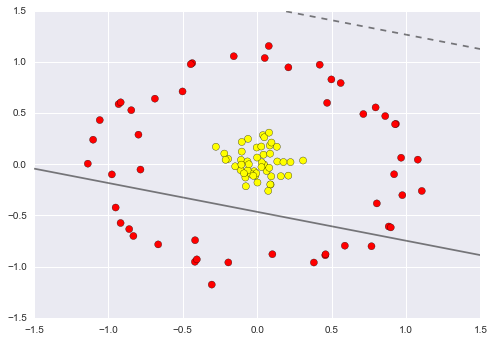
\includegraphics[width=0.9\linewidth]{Immagini/SVm non lineare.png}
		\captionsetup{width=.8\linewidth}
		\centering
		\caption{Punti originali rappresentando con i colori le categorie, con
		la linea solida il tentativo di tracciare un iperpiano e la linea
		tratteggiata il relativo margine. (fonte \cite{Data science handbook})} 
	\end{subfigure}
	\begin{subfigure}[t]{0.5\textwidth}
		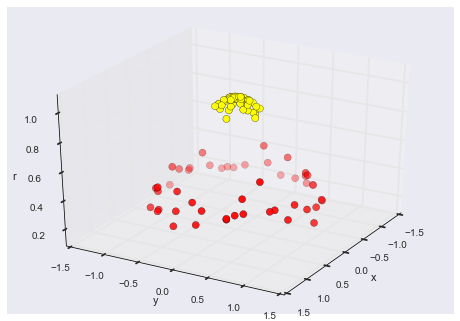
\includegraphics[width=0.9\linewidth]{Immagini/SVM kernel.png}
		\captionsetup{width=.8\linewidth}
		\centering
		\caption{Punti scalati mantenendo uguali le coordinate $x$ e $y$ e
		calcolando $z$ secondo $e^{-(x^2 + y^2)} + 1$ (fonte \cite{Data science handbook})}
\end{subfigure}

	
\end{figure}

Spesso però i dati reali non sono nettamente separabili e avremmo una zona in
cui dati di diverse categorie si sovrappongono. Per gestire al meglio questi
casi il modello ha un iperparametro $C$ che consente di specificare il grado di
rigidità del margine: con una $C$ molto grande avremmo una separazione molto
netta in cui nessun punto si trova all'interno del margine, al contrario con una
$C$ piccola permettiamo al modello di includere dei punti nel margine. $C$ è
utile anche per evitare che il nostro vettore sia troppo influenzato dalla
presenza di outlier: con un margine rigido l'iperpiano dovrà essere tracciato
massimizzando la sua distanza dall'outlier mentre ammettendo che questo ricada
all'interno del margine potremmo tracciare un iperpiano che massimizzi la
distanza dai dati reali.


\section{Alberi di decisione e foreste casuali}

\begin{figure}
	\centering
	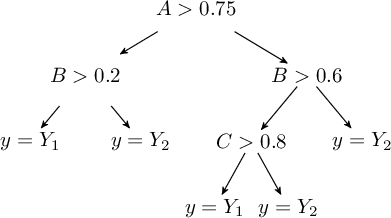
\includegraphics[width = 0.4\textwidth]{Immagini/Albero di decisione.png}
	\caption{Esempio di albero di decisione. Ad ogni nodo interno abbiamo una
	decisione basata su una caratteristica dei dati ($A$, $B$ e $C$) confrontata
	con un valore di soglia. Alle foglie invece abbiamo l'associazione con una
	categoria ($Y_1$ o $Y_2$)(fonte \cite{immagine albero
	decisione})}
\end{figure}

% L'obbiettivo è costruire un albero di decisione ovvero un albero in cui a ogni
% nodo in base al valore di una caratteristica del dato il processo di
% classificazione procede lungo uno dei sotto alberi fino a arrivare a una foglia
% che stabilisce la categoria del dato.

L'obbiettivo è generare un albero di decisione in grado di separare i dati nelle
corrette categorie. Un albero di decisione, come quello mostrato in figura 5,
non è altro che un albero binario in cui i nodi interni contengono una funzione
booleana che confronta una caratteristica dei dati con un valore di soglia. Le
foglie invece corrispondono a una delle categorie del problema. I dati vengono
classificati separando a ogni nodo i dati che verificano la funzione da quelli
che la falsificano. I due gruppi di dati procedono nei due sottoalberi allo
stesso modo fino a raggiungere le foglie dove vengono etichettati con la
categoria corrispondente alla foglia che hanno raggiunto.

Perché l'algoritmo funzioni è quindi necessario scegliere un valore di soglia
che al meglio separi i dati nelle corrette categorie. Per fare questo ci
serviamo di un indice di eterogeneità statistica, come l'indice di Gini o
l'entropia, scegliendo il valore della soglia che massimizza l'omogeneità
media delle categorie nei due sottoinsiemi di dati prodotti dalla decisione
ovvero due gruppi tali che ognuno è il più vicino possibile a avere una sola
categoria di dati.

Un problema di questo approccio è che tende a fare overfitting ovvero creare un
albero troppo adattato ai dati di training che poi non classifica correttamente
i dati reali soprattutto aumentando troppo la profondità dell'albero. Per
risolvere questo problema possiamo modificare i valori degli iperparametri come
la profondità massima o il numero minimo di dati per foglia oppure possiamo
usare un'altra tecnica: le foreste casuali. Le foreste casuali sono un
classificatore che aggrega una serie di alberi di decisioni prendendo la
classificazione più frequente tra questi. Per realizzarlo vengono allenati più
alberi di decisione con diversi sottoinsiemi dei dati di training e la
classificazione finale sarà ottenuta prendendo la classificazione più frequente
tra i diversi alberi di decisione.

\section{Naive Bayes}

Naive Bayes si basa sull'applicazione del teorema di Bayes:
$$
P(Y=y \mid X_1=x_1, \dots, X_n=x_n) = \frac{P(Y=y) P(X_1=x_1, \dots, X_n=x_n \mid Y=y)}
                                 				{P(X_1=x_1, \dots, X_n=x_n)},
$$

\noindent dove $Y = y$ è l'evento che si verifica quando la categoria corretta
del dato è $y$ e per $i = 1, ..., n$, $X_i = x_i$ è l'evento che si verifica
quando la $i$-esima caratteristica del dato da classificare assume il valore
$x_i$.

% Una delle
% ipotesi del teorema è  che le variabili $X_i \dots X_n$ siano tra loro indipendenti, questo non è
% sempre vero ma in problemi reali si può tipicamente assumerlo come vero e
% ottenere comunque buoni risultati.

Per assegnare una categoria a un dato dovremmo quindi trovare la categoria $y$
che massimizza la probabilità. Per fare questo possiamo stimare $P(Y = y)$, $P(X_1 = x_1 \mid Y = y), \dots, P(X_n = x_n \mid Y
= y)$ dalle frequenze del training set e ignorare $P(X_1=x_1, \dots, X_n=x_n)$
in quanto non dipende da $y$ e quindi massimizzare il numeratore è uguale a
massimizzare l'intera funzione. 

Questo approccio si basa su due importanti assunzioni: la prima è che le
variabili $X_i \dots X_n$ siano tra loro indipendenti, la seconda che abbiamo
abbastanza dati perché la frequenza delle probabilità nel training set sia
sufficientemente precisa nello stimare le probabilità reali. Seppure non abbiamo
prova di queste assunzioni spesso con dati reali riusciamo a ottenere un buon
stimatore anche se le ipotesi non sono del tutto vere.

\section{K-means}

K-means è l'unico algoritmo non supervisionato usato in questo progetto e si
basa sul dividere il training set in $K$ categorie scegliendo $K$ punti detti
baricentri e assegnando ogni dato alla categoria del baricentro più vicino. La
posizione dei baricentri viene ottimizzata cercando di minimizzare la somma
delle distanze quadratiche tra i dati del training set e il loro baricentro più
vicino. Quindi, formalmente, minimizziamo la quantità:
$$
\sum_{i=0}^{N}\min_{\mu_j \in C}(||x_i - \mu_j||^2),
$$

dove $N$ è il numero di dati di training, $C$ è l'insieme dei baricentri,
$\mu_j$ è quindi il $j$-esimo baricentro e $x_i$ è l'$i$-esimo dato.

Essendo questo un algoritmo non supervisionato non è nota l'associazione tra
baricentro e categoria reale e sarà quindi necessario ristabilire questa
associazione ad esempio associando ogni baricentro alla categoria più presente
nel suo insieme. Questa associazione non sarà sempre uno a uno infatti potrebbe
essere vantaggioso avere più baricentri che categorie reali associando più
baricentri alla stessa categoria.

\section{Conclusione} %TODO: pensare meglio al nome
In questo capitolo abbiamo introdotto in generale il machine learning e abbiamo
descritto i modelli usati in questo progetto: reti neurali, K-nearest neighbors,
macchine a vettori di supporto, alberi di decisione, foreste casuali, naive
bayes e K-means. Nel prossimo capitolo vedremo come questi concetti sono stati
applicati a un problema reale: classificare dei reperti archeologici in base
alla loro provenienza geografica. Vedremo in più dettaglio la natura del
problema oltre che alle tecniche utilizzate per risolverlo e per valutare la
bontà della soluzione trovata.
% 
% 
%			CAPITOLO 2: Il problema affrontato
\chapter{Il problema affrontato}
\label{cap2}
\section{Descrizione dei dati}
I dati consistono in una serie di misurazioni fatte su reperti archeologici. Per
ognuno di questi reperti sono state fate più misurazioni in punti diversi e
ognuna di questi ci dice la composizione dell'oggetto ovvero le percentuali di
potassio, calcio, titanio, cromio, manganese, ferro e zinco presente in quel
punto dell'reperto normalizzate in modo che la loro somma arrivi al 100\%
ottenendo così dati con sette caratteristiche. 

Di una parte di questi reperti conosciamo l'origine ovvero sappiamo se il
reperto è originario di tarquinia, luogo dove è stato ritrovato, o meno. Al
contrario per altri reperti questa informazione è sconosciuta e il nostro
obbiettivo è proprio di riuscire a trovarla.

In totale abbiamo 33 reperti con l'origine conosciuta, 24 dei quali di tarquinia
e 9 non, per un totale di 114 misurazioni. I reperti con origine sconosciuta
sono invece 78 con 132 misurazioni.

\section{Ambiente software}
Il progetto è stato svolto in python e tramite la libreria scikit-learn. Il
codice in se è scritto all'interno di notebook jupyter: dei file che consento di
scrivere celle di codice eseguibili singolarmente dividendo il programma in
passi più facilmente modificabili e rendendo più facile visualizzare cosa sta
facendo il programma. La libreria principale a cui gira attorno il progetto è
scikit-learn una libreria che contiene una serie di algoritmi di machine
learning oltre che alcune funzionalità di supporto all'utilizzo di questi
algoritmi. Tutti gli algoritmi descritti nel capitolo uno sono stati utilizzati
tramite funzioni fornite da scikit-learn così come le tecniche di testing che
vedremo nelle prossime sezioni. 

Sono poi state usate altre librerie in minor modo come pandas per la lettura e
scrittura di file excel, matplotlib per la creazione di alcuni grafici e joblib
per salvare i modelli allenati su disco. Il codice non dovrebbe richiedere una
versione specifica di python o di queste libreria ma per l'utilizzo dei modelli
salvati è necessario che python sia alla versione 3.7 e le librerie nelle
versioni specificate nel file requirements.txt.

\section{Repeated holdout}
Per holdout si intende la tecnica di valutazione di un algoritmo basata sul
separare i dati disponibili in un insieme di training e uno di testing. Il primo
insieme verrà usato per allenare il modello, il secondo per valutarlo.

Nonostante questa tecnica ci porti ad allenare il modello con meno dati avere
dei dati che il modello non hai mai visto ci permette di valutarlo più
accuratamente. Una parte importante della creazione di un modello è infatti la
sua valutazione: ci serve un modo per sapere se il modello creato funziona come
vorremmo e se l'algoritmo usato e gli iperparametri scelti sono adatti al nostro
problema.

Per repeated holdout non si intende altro che la ripetizione dell'hold out: a
ogni iterazione vengono randomizzati l'insieme di training e quello di testing e
viene ripetuto l'allenamento e la valutazione. La speranza è che facendo più
prove sempre con dati leggermente diversi riusciamo meglio a prevedere la
prestazione in tutte le istanze possibili del problema.

Nel progetto questa tecnica è stata usata solamente durante il test iniziale
fatto con una rete neurale come studio di fattibilità. Infatti questa tecnica
richiede di perdere una buona percentuale dei dati durante l'allenamento per
questo nel resto del progetto abbiamo quasi esclusivamente usato la convalida
incrociata: una tecnica che consente di ottenere una buona valutazione del
modello senza sacrificare una così grande percentuale di dati. Nella prossima
sezione spiegherò in più dettaglio come questo è possibile.

\section{Convalida incrociata}

Una popolare alternativa all'holdout è la convalida incrociata: si dividono i
dati in $K$ sezioni a questo punto si fanno $K$ prove, ognuna delle quali
utilizzerà una diversa delle $K$ sezioni come test set e le rimanenti come
insieme di training. Questo ci permette di usare una più alta percentuali di
dati per allenare il modello rispetto all'holdout e riuscire comunque a fare
buone misurazioni, ad esempio in questo progetto abbiamo principalmente usato
$K=5$ utilizzando quindi l'80\% dei dati per il training ad ogni prova. Questo
viene al costo di un maggior costo computazionale rispetto all'holdout infatti
dovremmo riallenare il modello $K$ volte e questo richiede tempo ma con un
database relativamente semplice come il nostro ne vale la pena.

% Questo è stato il principale metodo di valutazione usato in questo progetto.

\section{Griglia di ricerca}
Come abbiamo visto nel primo capitolo tutti i modelli usati hanno una serie di
iperparametri da definire ma come facciamo a sapere quali sono i valori
migliori? Un buon metodo è usare una griglia di ricerca: scegliamo una serie di
valori candidati per ogni iperparametro e non facciamo altro che provare ogni
possibile combinazione di questi allenando e valutando il modello in ogni
possibile configurazione. Per la valutazione utilizziamo la convalida incrociata
per i motivi spiegati nella sezione precedente. Questo ci permette di misurare
le prestazioni del modello con ogni valore degli iperparametri e possiamo
selezionare quelli che mostrano i risultati migliori.

\section{Schema delle prove}
Inizialmente la prima prova fatta è stata quella di eseguire semplicemente il
modello di rete neurale di scikit-learn {\it "MPLClassifier"} e una macchina a
vettori di supporto {\it "SVC"}. I due algoritmi sono stati eseguiti
semplicemente con i parametri di default e senza separare i dati di training e
di testing ma il test è stato sufficiente per capire che il problema era
affrontabile: gia senza modificare gli iperparametri abbiamo ottenuto oltre il
95\% di accuratezza, un ottimo risultato anche tenendo conto dei risultati
esagerati dall'unione di test e training set.

Il prossimo passo è stato quello di cercare di ottimizzare gli iperparametri
della rete neurale usando una griglia di ricerca. I due parametri che abbiamo
fatto variare sono il numero di neuroni nello strato nascosto e la funzione di
attivazione. Per lo strato nascosto abbiamo provato sia con un singolo strato
contenente tra i due e i venti neuroni sia con due strati ognuno con fino a 9
neuroni. Mentre per la funzione di attivazione abbiamo provato la funzione
identità ($f(x) = x$), la funzione sigmoidea ($f(x) = \frac{1}{1 + e^{-x}}$), la
funzione tangente iperbolica ($f(x)=\tanh(x) = \frac {e^x - e^{-x}} {e^x +
e^{-x}}$) e la funzione relu ($f(x) = max(0, x)$). In diverse esecuzioni della
griglia di ricerca diverse configurazioni dei parametri risultavano migliori.
Abbiamo provato a eseguire più volte la prova osservando la frequenza con cui un
certo iperparametro risultava il migliore o la media dell'accuratezza raggiunta
dallo stesso ma anche così nessuna configurazione spiccava come migliore sulle
altre. Visti i risultati non proveremo più molteplici strati nascosti dato che
non sembrano migliorare il risultato e aggiungono molti casi da tesare nella
griglia di ricerca aumentando significativamente il tempo di calcolo.

Abbiamo poi proceduto a sperimentare con gli altri modelli. Per ogni
modello abbiamo selezionato gli iperparametri più importanti da testare creando
una griglia di ricerca per ognuno. Fatto questo abbiamo per ognuno eseguito una
convalidazione incrociata testando a ognuna delle $K$ prove tutti i parametri
della griglia di ricerca e valutando il modello migliore per accuratezza,
sensibilità e specificità. Questo ci ha permesso di confrontare i vari modelli al
di là di una particolare configurazione di parametri ottenendo i risultati
consultabili nella prima tabella.


\begin{table}
	\caption{Risultati dell'esperimento per confrontare i vari modelli}
	\rule{\textwidth}{0.25mm}

	\caption{Rete neurale}
	\begin{tabular}{|l|l|l|}
	\hline
                & Media     & Deviazione standard	\\ \hline
	Accuratezza & 0.8947	& 0.06795				\\ \hline
    Sensibilità & 0.9287	& 0.114					\\ \hline
    Specificità & 0.8		& 0.1633				\\ \hline
	\end{tabular}
	\\


	\caption{K nearest neighbors}
	\begin{tabular}{|l|l|l|}
	\hline
                & Media     & Deviazione standard	\\ \hline
	Accuratezza & 0.9477	& 0.04959				\\ \hline
    Sensibilità & 0.9522	& 0.06874				\\ \hline
    Specificità & 0.9333	& 0.1333				\\ \hline
	\end{tabular}
	\\


	\caption{Macchine a vettori di supporto}
	\begin{tabular}{|l|l|l|}
	\hline
                & Media     & Deviazione standard	\\ \hline
	Accuratezza & 0.9212	& 0.05538				\\ \hline
    Sensibilità & 0.9404	& 0.09114				\\ \hline
    Specificità & 0.8667	& 0.1633				\\ \hline
	\end{tabular}
	\\


	\caption{Alberi di decisione}
	\begin{tabular}{|l|l|l|}
	\hline
                & Media     & Deviazione standard	\\ \hline
	Accuratezza & 0.9129	& 0.08039				\\ \hline
    Sensibilità & 0.9037	& 0.1227				\\ \hline
    Specificità & 0.9333	& 0.1333				\\ \hline
	\end{tabular}
	\\


	\caption{Foresta casuale}
	\begin{tabular}{|l|l|l|}
	\hline
                & Media     & Deviazione standard	\\ \hline
	Accuratezza & 0.9818	& 0.03636				\\ \hline
    Sensibilità & 1.0		& 0.0					\\ \hline
    Specificità & 0.9333	& 0.1333				\\ \hline
	\end{tabular}
	\\


	\caption{Naive bayes}
	\begin{tabular}{|l|l|l|}
	\hline
                & Media     & Deviazione standard	\\ \hline
	Accuratezza & 1.0		& 0.0					\\ \hline
    Sensibilità & 1.0		& 0.0					\\ \hline
    Specificità & 1.0		& 0.0					\\ \hline
\end{tabular}
\end{table}


%TODO: trovare il modo di mettere i dati delle performance dei modelli

Come discusso nella descrizione dei dati il nostro database è composto da più
misurazioni dello stesso dato. Fino ad adesso abbiamo trattato ogni dato come
un valore singolo e separato dagli altri ma in realtà questo potrebbe rivelarsi
un problema: se i dati sono troppo simili tra loro i modelli potrebbero
adattarsi troppo ai dati di training producendo quindi buoni risultai durante
l'allenamento ma rivelandosi poi essere poco buono con i dati reali trovandosi
quindi in una situazione detta overfitting. Per verificare che questo non stesse
avvenendo abbiamo separato i dati selezionando per ogni reperto una misurazione
e utilizzando l'insieme così creato per allenare i modelli mentre il resto delle
misurazioni è stato usato per il testing. Abbiamo poi utilizzato questo insieme
di training per riallenare i modelli utilizzando la stessa griglia di ricerca
usata nell'esperimento precedente per selezionare gli iperparametri testando poi
i modelli con i rimanenti dati. Osservando i risultati osserviamo che
l'accuratezza di quasi tutti i modelli è di poco calata suggerendo quindi che
l'overfitting non è un problema e anzi eliminando le ripetizioni riduciamo di
molto i dati usabili nel training peggiorando quindi i modelli risultati.

%TOOD: dati della performance modelli senza ripetizioni
\begin{table}
\caption{Risultati dell'esperimento per confrontare i vari modelli}
\rule{\textwidth}{0.25mm}

\caption{Rete neurale}
\begin{tabular}{|l|l|}
\hline
			& Media     \\ \hline
Accuratezza & 0.9851    \\ \hline
Sensibilità &    1.0    \\ \hline
Specificità &   0.95    \\ \hline
\end{tabular}
\\

\caption{K nearest neigh4bors}
\begin{tabular}{|l|l|}
\hline
			& Media     \\ \hline
Accuratezza & 0.9851    \\ \hline
Sensibilità & 0.9787    \\ \hline
Specificità &    1.0    \\ \hline
\end{tabular}
\\


\caption{Macchine a vettori di supporto}
\begin{tabular}{|l|l|}
\hline
			& Media     \\ \hline
Accuratezza & 0.9212	\\ \hline
Sensibilità & 0.9404	\\ \hline
Specificità & 0.8667	\\ \hline
\end{tabular}
\\


\caption{Alberi di decisione}
\begin{tabular}{|l|l|}
\hline
			& Media     \\ \hline
Accuratezza & 0.8507    \\ \hline
Sensibilità & 0.8085    \\ \hline
Specificità &   0.95    \\ \hline
\end{tabular}
\\


\caption{Foresta casuale}
\begin{tabular}{|l|l|}
\hline
			& Media   	\\ \hline
Accuratezza & 1.0    	\\ \hline
Sensibilità & 1.0    	\\ \hline
Specificità & 1.0    	\\ \hline
\end{tabular}
\\


\caption{Naive bayes}
\begin{tabular}{|l|l|}
\hline
			& Media   \\ \hline
Accuratezza & 0.9851  \\ \hline
Sensibilità & 0.9787  \\ \hline
Specificità &    1.0  \\ \hline
\end{tabular}

\end{table}




% [X]	Prova iniziale nn 
% [X]	grid search nn 
% [X]	cv nn 
% [X]	confronto modelli con grid search cv
% [X]	test senza ripetizioni
% [ ]	risultato finale, excel database da classificare


% 
% 
%			CAPITOLO 3: Risultati
\chapter{Risultati}
\label{cap3}
\section{Valutazione combinata}

% 
% 
%			CAPITOLO 4: Conclusioni
% \chapter{Conclusioni}44
% \label{cap4}

%
%			BIBLIOGRAFIA
%
\begin{thebibliography}{00}
%
% \bibitem{gotti91}
% M. Gotti, I linguaggi specialistici, Firenze, La Nuova Italia, 1991.
%
\bibitem{Intro to nn}
D. Kriesel, A brief introduction to neural networks, disponible su
http://www.dkriesel.com, 2007. %Seguendo "how to cite" sul sito
%

% https://towardsdatascience.com/support-vector-machine-introduction-to-machine-learning-algorithms-934a444fca47
\bibitem{Data science handbook}
Jake VanderPlas, Python Data Science Handbook, O'Reilly Media, disponibile su
https://jakevdp.github.io/PythonDataScienceHandbook/, 2016

\bibitem{immagine neurone}
Ioannou Yani, Structural Priors in Deep Neural Networks, 10.17863/CAM.26357,
2017

\bibitem{immagine albero decisione}
Paolo Medici, Elementi di analisi per Visione Artificiale, disponibile su
http://www.ce.unipr.it/~medici/geometry/geometry.html, 2017


\end{thebibliography}
% 
\end{document}


 
